%!TEX TS-program = xelatex
%!TEX encoding = UTF-8 Unicode
% Awesome CV LaTeX Template for CV/Resume
%
% This template has been downloaded from:
% https://github.com/posquit0/Awesome-CV
%
% Author:
% Claud D. Park <posquit0.bj@gmail.com>
% http://www.posquit0.com
%
% Template license:
% CC BY-SA 4.0 (https://creativecommons.org/licenses/by-sa/4.0/)
%


%-------------------------------------------------------------------------------
% CONFIGURATIONS
%-------------------------------------------------------------------------------
% A4 paper size by default, use 'letterpaper' for US letter
\documentclass[11pt, a4paper]{awesome-cv}

\usepackage{float}
\usepackage{overpic}
\usepackage{tikz}
\usetikzlibrary{shapes.geometric}

% Configure page margins with geometry
\geometry{left=1.4cm, top=.8cm, right=1.4cm, bottom=1.8cm, footskip=.5cm}

% Color for highlights
% Awesome Colors: awesome-emerald, awesome-skyblue, awesome-red, awesome-pink, awesome-orange
%                 awesome-nephritis, awesome-concrete, awesome-darknight
\colorlet{awesome}{awesome-orange}
% Uncomment if you would like to specify your own color
% \definecolor{awesome}{HTML}{CA63A8}

% Colors for text
% Uncomment if you would like to specify your own color
% \definecolor{darktext}{HTML}{414141}
% \definecolor{text}{HTML}{333333}
% \definecolor{graytext}{HTML}{5D5D5D}
% \definecolor{lighttext}{HTML}{999999}
% \definecolor{sectiondivider}{HTML}{5D5D5D}

% Set false if you don't want to highlight section with awesome color
\setbool{acvSectionColorHighlight}{true}

% If you would like to change the social information separator from a pipe (|) to something else
\renewcommand{\acvHeaderSocialSep}{\quad\textbar\quad}

\hypersetup{
  pdftitle={Personal CV},
  pdfauthor={Tommaso Bocchietti},
  pdfsubject={Curriculum Vitae},
  pdfkeywords={}
}

%-------------------------------------------------------------------------------
%	PERSONAL INFORMATION
%	Comment any of the lines below if they are not required
%-------------------------------------------------------------------------------
% Available options: circle|rectangle,edge/noedge,left/right
% \photo[circle,noedge,left]{common/img/Profile}
\name{Tommaso}{Bocchietti}
\position{Mechatronics and Robotics MSc student}
\address{Via Montagnola 13, San Fermo della Battaglia, Como (IT)}

\email{tommaso.bocchietti@gmail.com}
\mobile{(+39) 342-501-6560}
\github{Bocchio01}
\homepage{www.bocchio.dev}
\linkedin{tommaso-bocchietti}
% \dateofbirth{March 1st, 2001}
% \gitlab{gitlab-id}
% \stackoverflow{SO-id}{SO-name}
% \twitter{@twit}
% \skype{skype-id}
% \reddit{reddit-id}
% \medium{medium-id}
% \kaggle{kaggle-id}
% \googlescholar{googlescholar-id}{name-to-display}
%% \firstname and \lastname will be used
% \googlescholar{googlescholar-id}{}
% \extrainfo{extra information}

\quote{``Get things done!''}

\newcommand{\companyname}{\textbf{Whom It May Concern} }
\newcommand{\stars}[2][fill=darktext,draw=darktext]{
\begin{tikzpicture}[baseline=-0.34em,#1]
\foreach \X in {1,...,5}
{
\pgfmathsetmacro{\xfill}{min(1,max(1+#2-\X,0))}
\path (\X*1em,0)
node[star,draw, ultra thin,star point height=0.23em,minimum size=0.75em,inner sep=0pt,
path picture={\fill (path picture bounding box.south west)
rectangle  ([xshift=\xfill*0.722em]path picture bounding box.north west);}]{};
}
\end{tikzpicture}}

%-------------------------------------------------------------------------------
\begin{document}

% Print the header with above personal information
% Give optional argument to change alignment(C: center, L: left, R: right)
\makecvheader[C]

% Print the footer with 3 arguments(<left>, <center>, <right>)
% Leave any of these blank if they are not needed
\makecvfooter
{\today}
{Tommaso Bocchietti~~~·~~~Curriculum Vitae}
{\thepage}


%-------------------------------------------------------------------------------
%	CV/RESUME CONTENT
%	Each section is imported separately, open each file in turn to modify content
%-------------------------------------------------------------------------------
\descriptionstyle{
    Enthusiastic mechanical engineer with a strong problem-solving mindset and excellent technical skills in software development. \\
    My hands-on experience has enabled me to develop a diverse portfolio of projects, resulting in a distinctive ability to tackle complex challenges with a structured and analytical approach.
    I am currently seeking opportunities in the space industry to leverage my technical expertise, grow professionally in a dynamic environment, and contribute to cutting-edge projects.
}

%-------------------------------------------------------------------------------
%	SECTION TITLE
%-------------------------------------------------------------------------------
\cvsection{Experience}


%-------------------------------------------------------------------------------
%	CONTENT
%-------------------------------------------------------------------------------
\begin{cventries}

  % %---------------------------------------------------------
  \cventry
  {Mechatronic Engineer} % Job title
  {Polimi Sailing Team} % Organization
  {Politecnico di Milano, Lombardy, Italy} % Location
  {Oct. 2023 - PRESENT} % Date(s)
  {
    \begin{cvitems} % Description(s) of tasks/responsibilities
      \item {Coded from scratch high performance NMEA0183 libraries.}
      \item {Worked with STM32 microcontrollers to create interfaces for the sensors and the control algorithms.}
    \end{cvitems}
  }

  %---------------------------------------------------------
  \cventry
  {Mapper} % Job title
  {Orienteering Como} % Organization
  {Lombardy, Italy} % Location
  {May. 2018 - PRESENT} % Date(s)
  {
    \begin{cvitems} % Description(s) of tasks/responsibilities
      \item {Responsible for the society's cartography.}
      \item {Drawn several new Orienteering maps using the International Symbols Specification.}
      \item {Handled many homologation iter with the official Italian Federation for this sport.}
      \item {Developed a cloud-based architecture to facilitate the access and use of the map archive to all the members of the society.}
    \end{cvitems}
  }

  %---------------------------------------------------------
  \cventry
  {Private teacher} % Job title
  {Self-Employed} % Organization
  {Online \& Como, Lombardy, Italy} % Location
  {Feb. 2018 - PRESENT} % Date(s)
  {
    \begin{cvitems} % Description(s) of tasks/responsibilities
      \item {Private lessons and support in scientific subjects for students facing challenges.}
      \item {Age of students ranged from 14 to 19 years old.}
    \end{cvitems}
  }

  %---------------------------------------------------------
  \cventry
  {Software developer} % Job title
  {Confedilizia Como} % Organization
  {Como, Lombardy, Italy} % Location
  {Apr. 2020 - Feb. 2021} % Date(s)
  {
    \begin{cvitems} % Description(s) of tasks/responsibilities
      \item {Responsible for the development and distribution of a new software needed by the association.}
      \item {Developed the computer software for the specific needs and requests from the client.}
      \item {Developed the web platform (front-end \& database) for the secure distribution of the software to requesting clients.}
    \end{cvitems}
  }

  %---------------------------------------------------------
  \cventry
  {Web Programmer} % Job title
  {Ennova Research} % Organization
  {Lomazzo, Lombardy, Italy} % Location
  {Jun. 2018} % Date(s)
  {
    \begin{cvitems} % Description(s) of tasks/responsibilities
      \item {Period of internship for the "Alternanza Scuola Lavoro" national project.}
      \item {Developed a dynamically generated web page using Node.js and JavaScript.}
    \end{cvitems}
  }
\end{cventries}

%-------------------------------------------------------------------------------
%	SECTION TITLE
%-------------------------------------------------------------------------------
\cvsection{Education}


%-------------------------------------------------------------------------------
%	CONTENT
%-------------------------------------------------------------------------------
\begin{cventries}

  %---------------------------------------------------------
  \cventry
  {Master's Degree in Mechanical Engineering (Field of Mechatronics and Robotics)} % Degree
  {Politecnico di Milano} % Institution
  {Milan, Lombardy, Italy} % Location
  {Sep. 2023 - PRESENT} % Date(s)
  { }

  %---------------------------------------------------------

  %---------------------------------------------------------
  \cventry
  {Bachelor's Degree in Mechanical Engineering} % Degree
  {Politecnico di Milano} % Institution
  {Milan, Lombardy, Italy} % Location
  {Sep. 2020 - Jul. 2023} % Date(s)
  {
    \begin{cvitems} % Description(s) bullet points
      \item {Selected for participating in the "Pro Hackin' Project 2023", in collaboration with "RIMAC Automobil"\\
                  Project task: Personal Transportation Vehicle - Sidewalk vehicle\\
                  Chosen by the company as the winning team}
      \item {Selected for competing at SWERC 2021 (A.Y.2020/21)}
      \item {Third place in an internal coding competition using MATLAB (A.Y.2020/21)}
    \end{cvitems}
  }

  %---------------------------------------------------------

  %---------------------------------------------------------
  \cventry
  {High School Diploma, Scientific} % Degree
  {Scientific High School "Paolo Giovio"} % Institution
  {Como, Lombardy, Italy} % Location
  {Sep. 2015 - Jun. 2020} % Date(s)
  {
    \begin{cvitems} % Description(s) bullet points
      \item {Italian Physics Olympiad: admitted to regional selection (Feb. 2019)}
      \item {Italian Informatics Olympiad: admitted to regional selection (Apr. 2019, Apr. 2018)}
      \item {Italian Mathematics Olympiad: admitted to local district selection (Feb. 2017)}
    \end{cvitems}
  }

  %---------------------------------------------------------
\end{cventries}

\vspace{-\acvSectionTopSkip}

\begin{minipage}[t]{0.60\textwidth}

  \cvsection{Skills}\\

  \begin{cvskills}

    \cvskill
    {Engineering \stars{4.0}}
    {MATLAB, Ansys Fluent (basic level)}

    \cvskill
    {3D CAD \stars{3.0}}
    {CATIA V5, SolidWorks, Inventor}

    \cvskill
    {Programming \stars{4.0}}
    {C/C++, PHP, MySQL, Java, Python}

  \end{cvskills}

\end{minipage}
%
\hfill
%
\begin{minipage}[t]{0.35\textwidth}

  \cvsection{Languages}\\

  \begin{cvskills}

    \cvskill
    {Italian}
    {Native}

    \cvskill
    {English}
    {Proficient}

    % \cvskill
    % {French}
    % {Beginner}

  \end{cvskills}

\end{minipage}

% Needed to correctly space vertically the successive section
\cvsection{Extracurricular Activity}

\begin{cventries}

    %---------------------------------------------------------
    \cventry
    {IT Technician}
    {Italian Orienteering Committee}
    {Italy}
    {11.2018 - PRESENT}
    {
        \begin{cvitems}
            \item {Organizational IT aid at major Italian Orienteering Events.}
            \item {5 Days of Italy (07.2022)}
            \item {International MeetingOfVenice (11.2018 - PRESENT)}
        \end{cvitems}
    }

    %---------------------------------------------------------
    \cventry
    {Events Organizer}
    {Orienteering Como}
    {Lombardy (IT)}
    {01.2017 - PRESENT}
    {
        \begin{cvitems}
            \item {Educational and promotional outings in the role of instructor (mainly for schools or local association).}
            \item {Organizer playing key roles (controller or course-setter) in smaller events such as promotional or regional competitions.}
        \end{cvitems}
    }

    %---------------------------------------------------------
    \cventry
    {Council Members}
    {Orienteering Como}
    {Villa Guardia, Como (IT)}
    {09.2021 - PRESENT}
    {
        \begin{cvitems}
            \item {Member since 02.2016}
            \item {Council Member since 09.2021}
        \end{cvitems}
    }

    %---------------------------------------------------------
    \cventry
    {Ball boy}
    {Tennis Como}
    {Como (IT)}
    {2012 - 2014}
    {
        \begin{cvitems}
            \item {Assisted the organization of the annual ATP Challenger tournament held in Como.}
            \item {Played the role of ball boy for the years 2012, 2013, and 2014.}
        \end{cvitems}
    }

\end{cventries}
%-------------------------------------------------------------------------------
%	SECTION TITLE
%-------------------------------------------------------------------------------
\cvsection{Honors \& Awards}


%-------------------------------------------------------------------------------
%	SUBSECTION TITLE
%-------------------------------------------------------------------------------
% \cvsubsection{International}


%-------------------------------------------------------------------------------
%	CONTENT
%-------------------------------------------------------------------------------
\begin{cvhonors}

  %---------------------------------------------------------
  \cvhonor
  {Merit Exemption} % Award
  {} % Event
  {Milan, Italy} % Location
  {2022} % Date(s)

  %---------------------------------------------------------
  \cvhonor
  {Best Freshman Award} % Award
  {} % Event
  {Milan, Italy} % Location
  {2021} % Date(s)

  %---------------------------------------------------------
\end{cvhonors}

\cvsection{Presentation}

\begin{cventries}

  %---------------------------------------------------------
  \cventry
  {Presenter for <CONTRATTI A CANONE CONCORDATO>}
  {Online Webinar by F.I.M.A.A COMO}
  {Online}
  {16.02.2021}
  {
    \begin{cvitems}
      \item {Explained the importance of a computer based system to efficiently generate the new type of real estate contract.}
      \item {Demonstrated the app developed for Confedilizia Como as a potential solution for compliance with new laws.}
    \end{cvitems}
  }

\end{cventries}
\cvsection{Certifications}

\begin{cvskills}

  %---------------------------------------------------------
  \cvskill
  {Arduino 90/100}
  {Official Arduino certification, obtained on 17.04.2024}

  %---------------------------------------------------------
  \cvskill
  {TOEFL 90/120}
  {Test of English as a Foreign Language, obtained on 23.08.2023}

  %---------------------------------------------------------
  \cvskill
  {TOEIC 975/990}
  {Test of English for International Communication, obtained on 12.07.2023}

\end{cvskills}

%-------------------------------------------------------------------------------
%	SECTION TITLE
%-------------------------------------------------------------------------------
\cvsection{Hobby \& Personal interests}


%-------------------------------------------------------------------------------
%	CONTENT
%-------------------------------------------------------------------------------
\begin{cvskills}

  %---------------------------------------------------------
  \cvskill
  {Projects} % Hobby
  {
    \begin{cvitems} % Description(s) bullet points
      \item {Gorlu the printer | Joppo the rotor | Model rockets}
      \item {\dots many more on my website \dots}
    \end{cvitems}
  }
  %---------------------------------------------------------

  %---------------------------------------------------------
  \cvskill
  {Bike travelling} % Hobby
  {
    \begin{cvitems} % Description(s) bullet points
      \item {Como - London, 1200km+ (Sept. 2021)}
      \item {Como - Barcelona, 1100km+ (Aug. 2023)}
    \end{cvitems}
  }
  %---------------------------------------------------------

  %---------------------------------------------------------
  \cvskill
  {Sports} % Hobby
  {
    \begin{cvitems} % Description(s) bullet points
      \item {Orienteering (practiced since 2016)}
      \item {Tennis (played for 8 years)}
    \end{cvitems}
  }
  %---------------------------------------------------------

  %---------------------------------------------------------
  \cvskill
  {Nature} % Hobby
  {
    \begin{cvitems} % Description(s) bullet points
      \item {Camping}
      \item {Mountain hiking}
    \end{cvitems}
  }
  %---------------------------------------------------------

\end{cvskills}
\cvsection{Projects}

\descriptionstyle{
  Selection (not exhaustive) of some projects I've worked on that relate to my academic, professional, and personal interests.\\
  I consider them as way to experiment, learn, and get a hands-on approach to engineering.
}

\begin{cventries}

  %---------------------------------------------------------
  \cventry
  {Most of the projects were done individually, at the explicit request of the professor.}
  {Academic Projects}
  {Politecnico di Milano, Milan (IT) \& University of Waterloo, Waterloo (CA)}
  {14.09.2020 - PRESENT}
  {
    \begin{cvitems}
      \item {\textbf{Topology Optimization of 2D truss structures}: implementation of optimization routines based on the CONLIN algorithm.}
      \item {\textbf{Structural Health Monitoring (SHM) as a multivariate outlier detection problem}: analysis of a tie-rods element subjected to both damage and environmental variability, by means of statistical indices as Mahalanobis Squared Distance (MSD) and Principal Component Analysis (PCA).}
      \item {\textbf{Drag Coefficient Analysis of a Model Rocket Using Ansys Fluent}: simulation of the flow around a model rocket to determine the drag coefficient and comparison with theoretical model.}
      \item {\textbf{Development of a 2D CFD solver in C/C++ for the solution of the Navier-Stokes equations for incompressible flows}: implementation of the SCGS and SIMPLE algorithms, with validation on the lid-driven cavity flow.}
      \item {\textbf{Implementation of a nonlinear Finite Element Analysis (FEA) solver}: implementation of the plasticity theory based on the radial return algorithm on top of a linear FEA solver.}
      \item {\textbf{Chip Scale Atomic Clocks (CSAC)}: analysis of the physics behind their operation and current state of the art, with a focus on MEMS/NEMS technology.}
      \item {\textbf{Laser/Material Interaction}: thermal analysis of the laser cutting process, with a focus on the vaporization and melt mechanisms.}
      \item {\textbf{Analysis of the electronic density for a given molecule}: visualization of the electronic density field of a molecule using MATLAB}
    \end{cvitems}
  }

  %---------------------------------------------------------
  \cventry
  {Pro Hackin' Project 2023, in partnership with RIMAC Automobili}
  {Personal Transportation Vehicle (Sidewalk vehicle)}
  {Politecnico di Milano, Milan (IT) \& RIMAC Automobili, Zagreb (HR)}
  {09.03.2023 - 01.06.2023}
  {
    \begin{minipage}{0.72\textwidth}
      \vspace{5pt}
      \begin{center}
        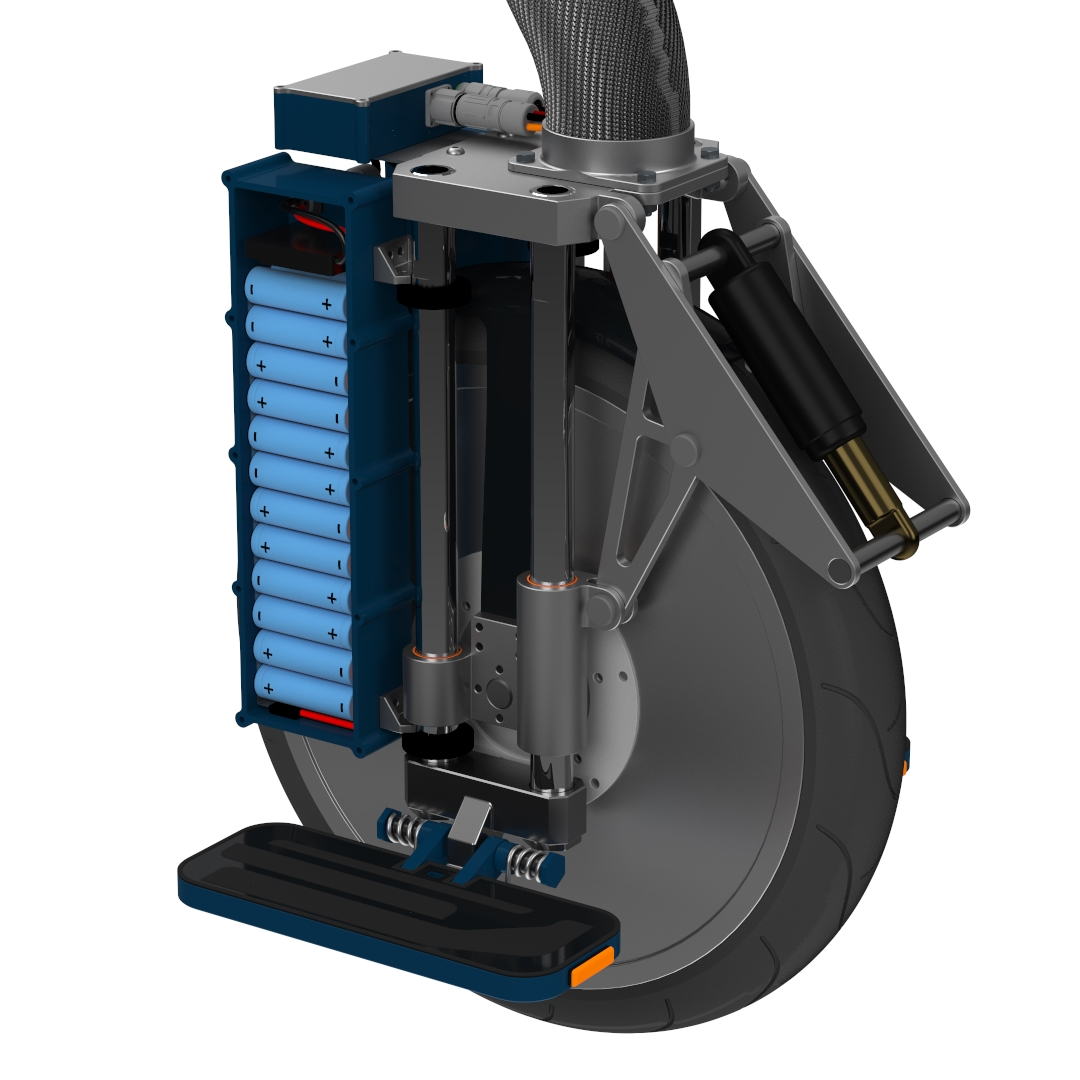
\includegraphics[height=120pt]{common/img/Rimac/1.jpg}
        \hspace{2cm}
        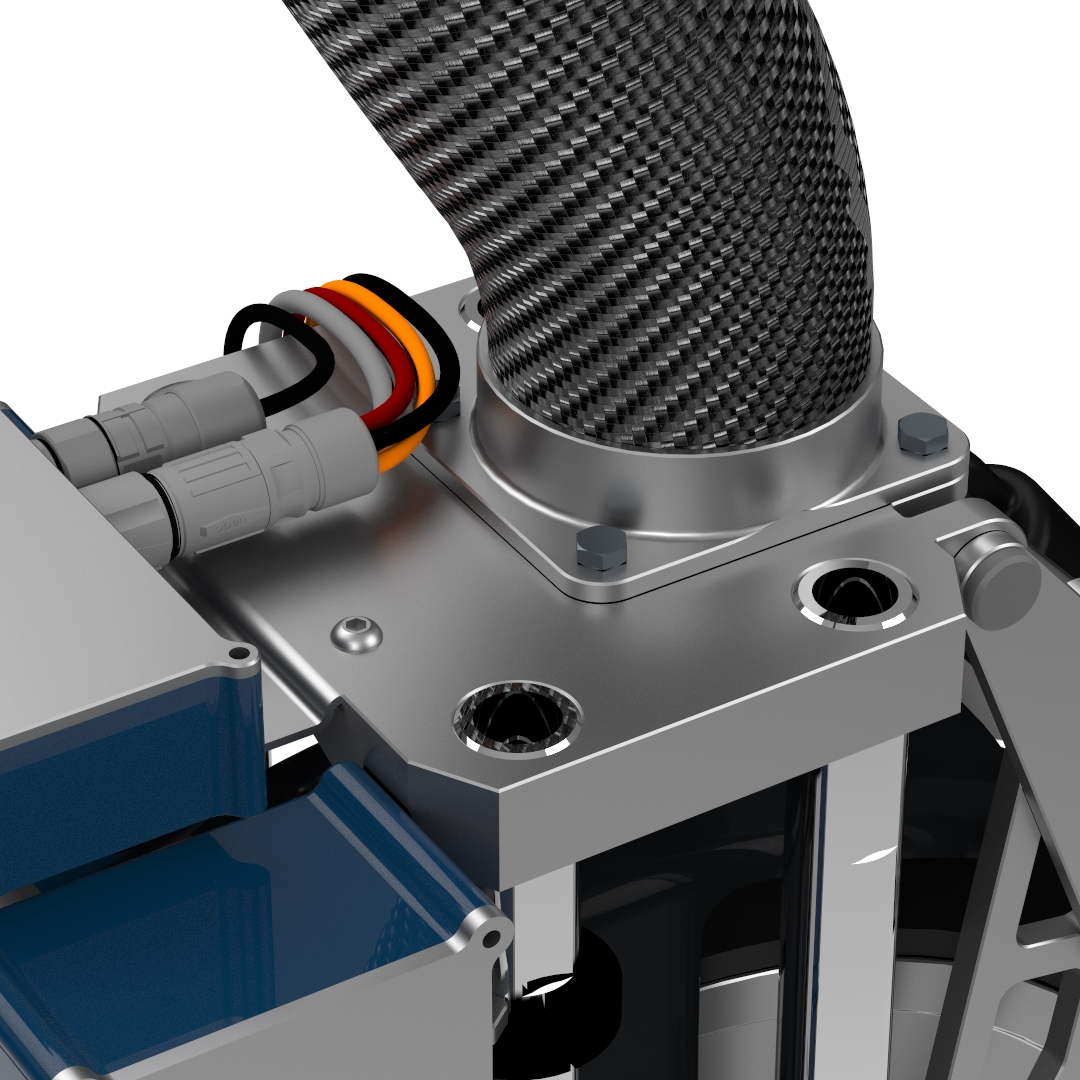
\includegraphics[height=120pt]{common/img/Rimac/2.jpg}
      \end{center}
      \vspace{5pt}
      Idealize and Design a Personal Transportation Vehicle (Sidewalk vehicle).\\
      Team-based project with students from 4 top European universities, featuring feedback sessions after each hackathon by company engineers. Selected as winning team.\\
      \begin{cvitems}
        \item {Hackathon 1: visions, user personas and functions \& requirements}
        \item {Hackathon 2: functional decomposition, morphological matrix and concepts development}
        \item {Hackathon 3: CAD design, FEM simulations, FMEA and cost analysis.}
      \end{cvitems}
      \vspace{4mm}
      \vspace{5pt}
    \end{minipage}
    \hfill
    \begin{minipage}{0.25\textwidth}
      \vspace{5pt}
      \begin{center}
        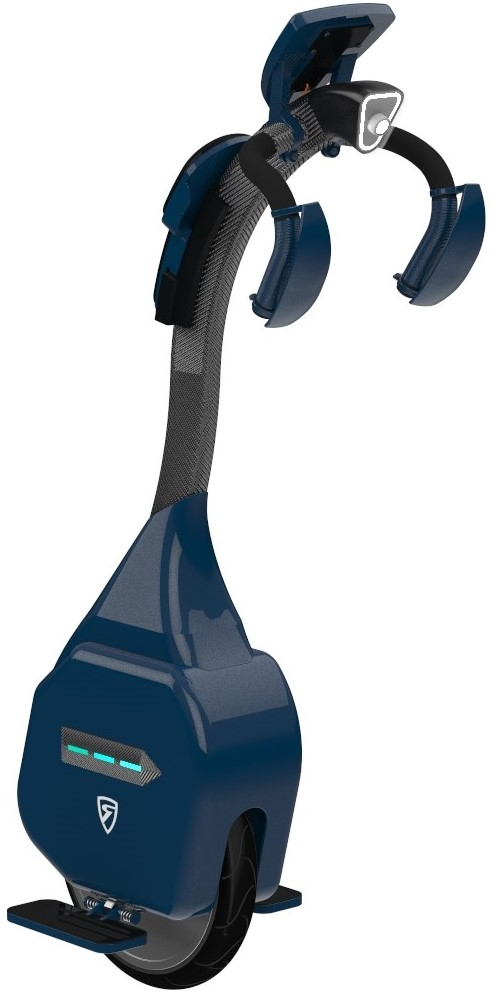
\includegraphics[height=200pt]{common/img/Rimac/3.jpg}
      \end{center}
      \vspace{5pt}
    \end{minipage}
  }

  %---------------------------------------------------------
  \cventry
  {Personal project to celebrate BSc}
  {Model Rocket with On-Board Flight Computer}
  {Personal Workshop, Como (IT)}
  {12.07.2023 - 21.07.2023}
  {
    \begin{minipage}{\textwidth}
      \vspace{5pt}
      \begin{overpic}[percent, width=\textwidth]{common/img/Rocket/Rocket.png}
        \put(4, 1.5){\subentrydatestyle{Fully functional flight computer in $< 20cm^3$}}
        \put(53, 1.5){\subentrydatestyle{Simulations driven design ($C_D \approx 0.806$)}}
        \put(19, 9.5){\subentrydatestyle{Launched and recovered without any damage, maximum elevation $+538m$}}
      \end{overpic}
      \vspace{3pt}
      Designing, optimization and building of a $63cm$ model rocket.\\
      Final design was achieved after a couple of iterations between CAD model and CFD simulations.
      Built mostly from cheap materials (cardboard \& wood) and 3D printed parts (PLA based).
      Essential characteristics:\\
      \begin{cvitems}
        \item {Flight time $\approx 60s$, maximum speed reached $+120m/s$, maximum acceleration $+10g$.}
        \item {Recovery system based on parachute, fully functional and reliable.}
        \item {On board flight computer with barometric, temperature and acceleration sensors capable of logging data.}
      \end{cvitems}
      \vspace{4mm}
    \end{minipage}
  }

  %---------------------------------------------------------
  \cventry
  {Done for fun or for educational purposes}
  {Selection of other minor projects}
  {Personal Workshop, Como (IT)}
  {2021 - PRESENT}
  {
    \begin{minipage}{0.45\textwidth}
      \vspace{5pt}
      \begin{center}
        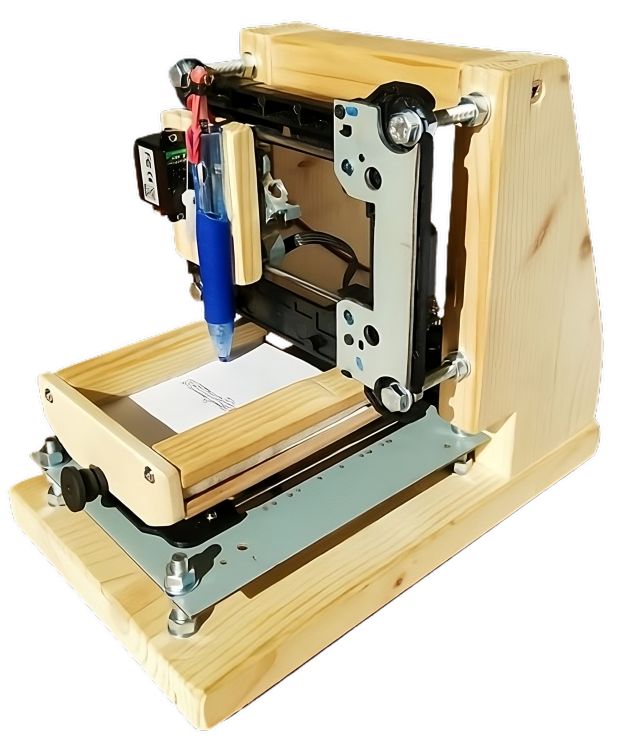
\includegraphics[height=150pt]{common/img/Minors/Gorlu.png}
        \hspace{4cm}
      \end{center}
      \vspace{5pt}
      CNC plotter to go from any digital image to its physical representation.\\
      \begin{cvitems}
        \item {Arduino based plotter with custom software.}
        \item {Canny edge detection algorithm.}
        \item {Recycled components from old DVD drives and wood.}
      \end{cvitems}
      \vspace{4mm}
      \vspace{5pt}
    \end{minipage}
    \hfill
    \begin{minipage}{0.45\textwidth}
      \vspace{5pt}
      \begin{center}
        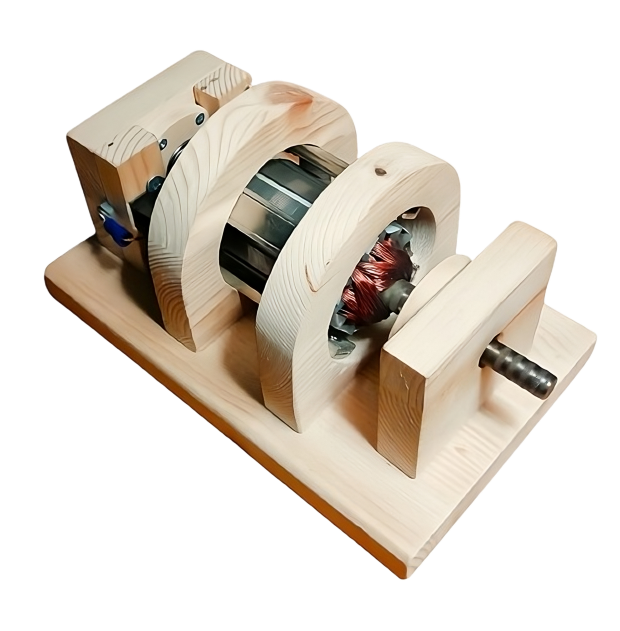
\includegraphics[height=150pt]{common/img/Minors/Joppo.png}
        \hspace{4cm}
      \end{center}
      \vspace{5pt}
      DC electric motor model to explain its working principle to my peer students.\\
      \begin{cvitems}
        \item {Recycled components from an old lawn mower and wood.}
        \item {Controllable in speed via a custom electrical circuit (diodes bridge and potentiometer).}
      \end{cvitems}
      \vspace{4mm}
      \vspace{5pt}
    \end{minipage}
  }

\end{cventries}

% Signature and data treatment
\vspace*{\fill}

\begin{flushright}
  \descriptionstyle{\textit{Tommaso Bocchietti}}

  
\includegraphics[width=0.25\textwidth]{common/img/Signature.png} \vspace{-4mm} \\
  \rule{0.27\textwidth}{0.5pt}
\end{flushright}

\begin{center}
  \footerstyle{I hereby give consent for my data included in this document to be processed by \companyname for recruiting purposes.}
\end{center}

%-------------------------------------------------------------------------------
\end{document}
